\documentclass[paper=a4, fontsize=11pt,twoside]{article}

% --------------------------------------------------------------------
% General Page Layout
% --------------------------------------------------------------------
\usepackage[a4paper]{geometry}
\usepackage[parfill]{parskip}
\setlength{\oddsidemargin}{5mm}		% Remove 'twosided' indentation
\setlength{\evensidemargin}{5mm}
\setlength{\parindent}{1mm}
\setlength{\parskip}{1mm}
%%
% --------------------------------------------------------------------
% Encoding and Language Settings
% --------------------------------------------------------------------
\usepackage[T1]{fontenc}
\usepackage[utf8]{inputenc}			% encoding may need to be changed depending on the system
\usepackage[swedish]{babel}
\usepackage{lipsum}					% Lorem Ipsum

% --------------------------------------------------------------------
% Utilities (colors, links, pictures, ect...)
% --------------------------------------------------------------------
\usepackage{xcolor}
\usepackage{hyperref}
\usepackage{graphicx}
\usepackage{amssymb}
\usepackage{epstopdf}
\usepackage[round]{natbib}
\usepackage{float}
\DeclareGraphicsRule{.tif}{png}{.png}{`convert #1 `dirname #1`/`basename #1 .tif`.png}

% -------------------------------------------------------------------------------------------------------------%
% Title Page / Document Class Definitions (Please Don't Play With This)			%
% -------------------------------------------------------------------------------------------------------------%
%
% Horizontal rule													%
\newcommand{\HRule}[1]{\rule{\linewidth}{#1}}   							%
%
% Document Number												%
\newcommand{\documentNumber}[1]{\centering PUSP1742#1 \\[1.0cm]}	 		%
%
% Document Version													%
\newcommand{\documentVersion}[1]{\centering \small{v.#1} \\[1.0cm]}	 		%
%
% Title															%
\makeatletter                           											%
\def\printtitle{%                       											%
	{\centering \@title\par}}												%
\makeatother                                    										%
%
% Author															%
\makeatletter                           											%
\def\printauthor{%                  											%
	{\centering \large \@author}}               									%
\makeatother														%
%
\newcommand{\grouptitlepage}[4]{										%
	\title{ 														%
		\documentNumber{#1}											%
		\documentVersion{#2}											%
		\HRule{0.5pt} \\ % Upper rule										%
		\LARGE \textbf{\uppercase{#3}} \\  									%
		\large \textbf{\uppercase{ETSF20 Grupp 2}}							%
		\HRule{2pt} \\ [0.5cm]      	% Lower rule + 0.5cm spacing					%
		\normalsize          		% Todays date								%
	}															%
	\author{#4}													%
	\maketitle														%
	\tableofcontents												%
	\thispagestyle{empty} 											%
	\newpage														%
}																%
%
% -------------------------------------------------------------------------------------------------------------%
% Title Page / Document Class Definitions (Please Don't Play With This)			%
% -------------------------------------------------------------------------------------------------------------%
\date{}                                           	% Activate to display a given date or no date


% -------------------------------------------------------------------------------------------------------------
% DOCUMENT START (YOU CAN IGNORE EVERYTHING ABOVE HERE)					
% -------------------------------------------------------------------------------------------------------------
\begin{document}
	
	% ---------------------------------------------------------------------------------------------------------------------------------------
	% Title Page START: \grouptitlepage{doc number}{Version Number}{doc title}{group responsible for doc}		
	% ---------------------------------------------------------------------------------------------------------------------------------------
	\grouptitlepage
	%Document Code Number (same as time reports)
	{12	}
	%Document Version Number										
	{0.1}
	%Document Title		Dokumentmall							
	{System Requirements Specifikation}
	%Group Responsible For Document									
	{(SG) System Grupp: \\ Benjamin Holmqvist \\ Carl rikner \\Marlina Degirmenci}	
	% -------------------------------------------------------------------------------------------------------------
	% Title Page END				
	% -------------------------------------------------------------------------------------------------------------
	\section{Introduktion}
	Detta dokument beskriver kraven för ett tidrapporteringssystem, baserat på “BaseBlockSystem”. Det är ett system där man främst kan skapa och lagra tidrapporter för enskilda medlemmar i ett projekt. Se referens dokumentet nedan för mer ingående förklaring av systemet.
	\section{Referensdokument}
	Base block System SRS: \textbf{\textit{PUSS12002 version: 1.0}}  gäller för alla punkter. Det som står i detta dokument gäller om det inte är specificerat i respektive underrubrik att det som står i \textbf{\textit{PUSS12002 version: 1.0}}  utgår för specifik del.
	
	\section{Bakgrund och Mål}
	
	\subsection{Huvudmål:}
	Det huvudsakliga målet med systemet är att erbjuda ett funktionellt tidrapporteringssystem som bygger vidare på ett redan givet “BaseBlockSystem”. Systemet ska kunna användas av projektgrupper för att enkelt kunna rapportera in arbetstid.
	\subsection{Aktörer och deras mål:}
	Följande huvudaktörer använder systemet:
	\subsubsection{Användare:}
	En användare ska ha en roll i projektgruppen. Den ska kunna tidrapportera, ändra en osignerad tidrapport. Användaren ska kunna se en sammanställning av sin totala rapporterade tid. Det huvudsakliga målet för en användare är att på ett simpelt sätt kunna tidrapportera.
	\subsubsection{Projektledare:}
	En projektledare är en specifik användare som har tilldelats rollen “Projektledare” av administratören. En projektledare ska, utöver det som en användare kan göra, kunna tilldela de olika rollerna till användarna. Projektledare ska kunna signera och annullera rapporter från övriga projektmedlemmar. Projektledaren ska kunna se en sammanställning av all den totala tid som rapporterats in i projektet. De huvudsakliga målen för en projektledare är att kunna rapportera tid, signera tidrapporter och tilldela roller till projektmedlemmarna. 
	\subsubsection{Administratör:}
	En administratör ska kunna lägga till och ta bort användare i systemet. Den ska även kunna tilldela rollen “Projektledare” till användare. Administratören ska kunna skapa och ta bort projektgrupper samt kunna tilldela användare till dessa projektgrupper. De huvudsakliga målen för en administratör är att kunna lägga till och ta bort användare, lägga till och ta bort projektgrupper samt kunna tilldela rollen “Projektledare”.
	
	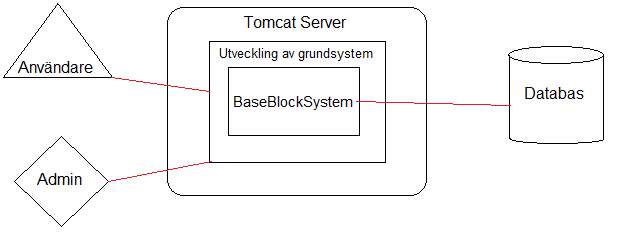
\includegraphics{kontextdiagram_SRS.png}
	
	\section{Terminologi}
	\paragraph{Tidrapport}
	\flushleft
	Dokument som används för att rapportera de timmar som man har lagt på olika områden i ett arbete/projekt används i samband med löne- och projektredovisning.
	\paragraph{Administratör}
	\flushleft
	Någon som förvaltar en organisation. I detta projektets fall, ett system.
	\paragraph{Förvaltning}
	\flushleft
	Vara ansvarig för ett visst arbete till någons räkning, eller ha hand om en verksamhet.
	\paragraph{Annullera}
	\flushleft
	Upphäva, ogiltigförklara något, t.ex. annullera en signering av en tidrapport.
	\paragraph{Projekt}
	\flushleft
	Ett uppdrag som utförs av en viss arbetsorganisation för att åstadkomma ett visst resultat. 
	\paragraph{Signering}
	\flushleft
	Bekräftar en tidrapport och sätter den i ett stadie där den inte kan ändras om inte projektledare häver signeringen.
	\paragraph{}
	\newpage
	\section{Kontext Diagram}
	Ett kontextdiagram kan ses i figur 1.
	
	\section{Funktionella Krav}
	
	\subsection{Administratör:}
	\subsubsection{Krav:}
	När en administratör vill ta bort en projektgrupp ska en varningsruta visas som frågar om admin vill ta bort projektgruppen.
	
	\subsubsection{Krav:} Följande scenario ska stödjas av systemet.
	\paragraph{Scenario:}
	Admin vill lägga till en projektgrupp i systemet.
	\paragraph{Förkrav:}
	Admin är inloggad.
	\paragraph{}
	\begin{enumerate}
		\item Admin går till sidan för hantering av projektgrupper
		\item Admin väljer att lägga till en projektgrupp
		\item Admin uppmanas att mata in ett namn på projektgruppen
		\item Projektgruppen skapas
		\item Admin ser en uppdatering av sidan
	\end{enumerate}
	
	\subsubsection{Krav:} 
	Följande scenario ska stödjas av systemet.
	\paragraph{Scenario:}
	Admin vill ta bort minst en projektgrupp i systemet.
	\paragraph{Förkrav:}
	Admin är inloggad. Det finns minst en projektgrupp.
	\paragraph{}
	\begin{enumerate}
		\item Admin går till sidan för hantering av projektgrupper
		\item Admin markerar vilken/vilka projektgrupper som ska tas bort
		\item Projektgruppen/grupperna som valts raderas
		\item Admin ser en uppdatering av sidan
	\end{enumerate}
	
	\subsubsection{Krav:} Följande scenario ska stödjas av systemet. 
	\paragraph{Scenario:}
	Admin skall utse projektledare i system utan användare.
	\paragraph{Förkrav:}
	Admin är inloggad. Ingen användare finns i systemet. Det finns minst en projektgrupp i systemet.
	\paragraph{}
	\begin{enumerate}
		\item Admin går till sidan för hantering av medlemmar
		\item Admin lägger till användare i en projektgrupp
		\item Admin tilldelar användaren rollen som projektledare
		\item Admin ser en uppdatering av sidan
	\end{enumerate}
	
	\subsubsection{Krav:} Följande scenario ska stödjas av systemet. 
	\paragraph{Scenario:}
	Admin skall utse projektledare med redan existerande användare i systemet.
	\paragraph{Förkrav:}
	Admin är inloggad. Det finns minst en användare i systemet. Det finns minst en projektgrupp i systemet.
	\paragraph{}
	\begin{enumerate}
		\item Admin går till sidan för hantering av användare
		\item Admin utser en användare och tilldelar denna rollen som projektledare
		\item Användaren har enbart rollen som projektledare
		\item Admin ser en uppdatering av sidan
	\end{enumerate}
	\newpage
	\subsubsection{Krav:} Följande scenario ska stödjas av systemet. 
	\paragraph{Scenario:}
	Admin vill lägga till en användare i systemet.
	\paragraph{Förkrav:}
	Admin är inloggad. 
	\paragraph{}
	\begin{enumerate}
		\item Admin går till sidan för hantering av användare
		\item Admin väljer att lägga till en användare
		\item Admin uppmanas att mata in namn på den nya användaren
		\item Admin uppmanas att mata in e-post som kopplas till den nya användaren
		\item Användaren skapas med valt användarnamn och e-post
		\item Användaren får e-post med användarnamn och slumpat lösenord
		\item Admin ser en uppdatering av sidan
	\end{enumerate}
	
	\subsubsection{Krav:} Admin ska kunna ta bort flera medlemmar samtidigt genom att kryssa i en ruta för vardera medlem som ska raderas. Sedan ska admin trycka på en knapp för att ta bort dessa.
	\subsubsection{Krav:} Admin ska inte kunna ta bort sig själv.
	
	\subsubsection{Krav:} Följande scenario ska stödjas av systemet. 
	\paragraph{Scenario:}
	Admin vill ta bort användare i systemet.
	\paragraph{Förkrav:}
	Admin är inloggad. Det finns minst en användare i systemet.
	\paragraph{}
	\begin{enumerate}
		\item Admin går till sidan för hantering av användare
		\item admin markerar vilken/vilka användare som ska raderas
		\item Användarna raderas ur systemet
		\item Admin ser en uppdatering av sidan
	\end{enumerate}
	
%------------------------------------------------------------------------------------------------------------
%Projektledare start
%------------------------------------------------------------------------------------------------------------
\newpage
\subsection{Projektledare:}
\paragraph{}
\subsubsection{Krav:} En projektledare ska kunna tilldela roller till projektmedlemmarna i projektgruppen.

\paragraph{}
\subsubsection{Krav:}
Följande scenario ska stödjas av systemet
\paragraph{Scenario:}
Projektledarer tilldelar en roll till en projektmedlem.
\paragraph{Förkrav:}
Användaren är projektledare i projektgruppen.
\begin{enumerate} 
\item Projektledare klickar på "Main"
\item Projektledare klickar vidare på "Organize group"
\item En ny sida visas med en lista på medlemmar i projektgruppen.
\item Projektledare klickar på roll-alternativ för den medlem som ändringen gäller
\item Projektledare ändrar/tilldelar rollen
\item Tryck på knappen “Update group”
\end{enumerate}

\paragraph{}
\subsubsection{Krav:}
	Projektledaren kan inte kunna tilldela mer än en roll till en medlem i projektgruppen.

\paragraph{}
\subsubsection{Krav:}
	Projektledaren ska kunna ändra projektmedlemmarnas roller i projektgruppen.
\paragraph{}
\newpage
\subsubsection{Krav:}
De roller som ska finnas tillgängliga är som följande:
\begin{itemize}
\item Projektgrupp
\item Systemgrupp
\item Utvecklingsgrupp
\item Testgrupp
\end{itemize}

\paragraph{}
\subsubsection{Krav:}
Projektledaren ska kunna signera och godkänna tidrapporter för varje medlem i gruppen.

\paragraph{}

\subsubsection{Krav:}
Följande scenario ska stödjas av systemet.
\paragraph{Scenario:}
Projektledare ska signera veckorapporter.
\paragraph{Förkrav:}
Användaren är projektledare i gruppen.
\begin{enumerate}
\item Projektledaren klickar på “Time Reporting”
\item Projektledaren klickar på “Sign Time Reports”
\item En lista kommer upp med alla Veckorapporter
\item Projektledaren markerar rapporterna som ska signeras och klickar på knappen “Sign”
\item När Projektledaren har signerat rapporterna kommer den tillbaka till en uppdaterad lista av rapporterna
\end{enumerate}

\paragraph{}

\subsubsection{Krav:}
Signeringen av tidrapport sker veckovis.

\paragraph{}

\subsubsection{Krav:}
Projektledarens egna tidrapport signeras direkt vid tryckning av submit-knappen.

\paragraph{}

\subsubsection{Krav:}
Listan för veckorapporter ska innehålla namn, rapporterad tid per aktivitet, veckonummer, grupptillhörighet och en kryssruta per rapport.

\paragraph{}

\subsubsection{Krav:}
Följande scenario ska stödjas av systemet.
\paragraph{Scenario:} Annullering av redan signerad tidrapport.
\paragraph{Förkrav:} Projektledaren är inloggad.
\begin{enumerate}
\item Projektledaren klickar på “Time reporting”
\item Projektledaren klickar på “Unsign reports”
\item Projektledaren kryssar för de signerade rapporterna som ska annulleras
\item Projektledaren klickar sedan på “Submit changes”
\end{enumerate}

\paragraph{}

\subsubsection{Krav:}
 Projektledaren ska, i menyn, ha följande länkar:
 \begin{itemize}
 \item “Organize Group”
 \item “Sign reports”
 \item “Unsign reports”
 \item “View all reports”
 \end{itemize}

\paragraph{}

\subsubsection{Krav:}
Projektledare ska kunna generera sammanställning över all tid som rapporterats i projektet.
\paragraph{-}
Sammanställningen ska kunna användas för att producera en sammanställning av statistik.

\newpage
\subsubsection{Krav:}
Projektledaren ska kunna se statistik för tidrapporter i projektet för varje medlem.
\paragraph{}
Tidrapporter ska kunna summeras och visas per:
\begin{itemize}
\item Användare
\item Roll
\item Aktivitet
\item Vecka
\end{itemize}
%---------------------------------------------------------------------------------------------------------
%Projektledare slut
%---------------------------------------------------------------------------------------------------------

	\subsection{Användare:}
	\subsubsection{Krav:} En användare ska kunna tidrapportera till det projekt som den är medlem i.
	\subsubsection{Krav:} Följande scenario ska stödjas av systemet.
	\paragraph{Scenario:} En användare vill skriva en tidrapport.
	\paragraph{Förkrav:}
	Användaren är inloggad i systemet.
	
	\begin{enumerate}
		\item	Användaren är inloggad i systemet
		\item 	Användaren går till sidan för hantering av tidrapport
		\item 	Användaren fyller i aktuella tider för de olika aktiviteterna. Fält lämnas tomma om ingen tid har lagts på aktiviteten.
		\item	Användaren väljer att skicka tidrapporten
		\item 	Tidrapporten skickas till projektledaren för signering
		\item 	Användaren ser en uppdatering av sidan
		
		
	\end{enumerate}
	
	\subsubsection{Krav:} En användare som är medlem i ett projekt ska kunna uppdatera osignerade tidrapporter i det projektet.
	\subsubsection{Krav:} En användare som är medlem i ett projekt ska kunna ta bort osignerade tidrapporter i det projektet.
	\subsubsection{Krav:} En användare ska kunna se all den tid som användaren har rapporterat.
	\subsubsection{Krav:} En användare får endast ha en eller ingen roll i projektgruppen.
	\subsubsection{Krav:} Följande scenario ska stödjas av systemet.
	\paragraph{Scenario:} Användaren vill uppdatera sin tidrapport
	\paragraph{Förkrav:}
	Användaren är inloggad i systemet och användarens tidrapport är osignerad.
	\begin{enumerate}
		\item	Användaren klickar på “Time Reporting”
		\item	Användaren klickar på “Edit time report”
		\item	Användaren kommer till en sida som innehåller en meny med användarens osignerade tidrapporter
		\item 	Användaren klickar på en tidrapport
		\item	En sida öppnas som visar aktuell tidrapport i form av en tabell med de gamla värdena ifyllda
		\item	Användaren ändrar/lägger till värden i tidrapporten
		\item	Användaren klickar på “Submit Change”
		\item	Den gamla tidrapporten försvinner och den ändrade tidrapporten skickas vidare för signering
		\item	“Time Reporting” sidan visas
		
	\end{enumerate}
	\subsubsection{Krav:}Följande scenario ska stödjas av systemet.
	\paragraph{Scenario:}Användare vill se en sammanfattning av sin rapporterade tid.
	\paragraph{Förkrav:}
	Användaren är inloggad i systemet.
	\paragraph{}
	\begin{enumerate}
		\item  Användaren klickar på “Time Reporting” i menyn
		\item  En ny sida visas som innehåller alternativ för tidrapportering samt en sammanställning för den totalt rapporterade tiden för användaren i form av en tabell
		
	\end{enumerate}
	\newpage
	\subsubsection{Krav:} Följande scenario ska stödjas av systemet.
	\paragraph{Scenario:}Användaren vill ändra lösenord.
	\paragraph{Förkrav:}
	Användaren är inloggad i systemet.
	\paragraph{}
	\begin{enumerate}
		\item	Användaren trycker på “Change Password” i menyn
		\item	En sida visas som innehåller relevanta textfält
		\item	Användaren fyller i nuvarande lösenord i det första textfältet
		\item	Användaren fyller i det nya lösenordet i det andra textfältet
		\item	Användaren upprepar det nya lösenordet i det tredje textfältet
		\item	Användaren trycker på knappen “Change Password”
		\item	Lösenordet för användaren ändras i systemet. Detta visas på följande sida
		
	\end{enumerate}
	
	\subsubsection{Krav:}Följande scenario ska stödjas av systemet.
	\paragraph{Scenario:}Användaren vill ändra lösenord (ogiltig inmatning)
	\paragraph{Förkrav:}
	Användaren är inloggad i systemet.
	\paragraph{}
	\begin{enumerate}
		\item  Användaren trycker på “Change Password” i menyn
		\item	 En sida visas som innehåller relevanta textfält
		\item	Användaren fyller i nuvarande lösenord i det första textfältet
		\item	Användaren fyller i det nya lösenordet som inte uppfyller krav 6.2.3 i PUSS12002 version: 1.0 för “BaseBlockSystem” i det andra textfältet
		\item	Användaren upprepar det nya lösenordet i det tredje textfältet
		\item	Användaren trycker på knappen “Change Password”
		\item	Lösenordet ändras inte och ett felmeddelande visas
		\item Användaren skickas tillbaka till steg 2
		
	\end{enumerate}
	\newpage
	\section{Kvalitets Krav}
	Läs kap 7.0  “Base block System SRS”:   \textbf{\textit{PUSS12002 version: 1.0}} 
	\section{Projekt Krav}
	Läs kap 8.0  “Base block System SRS”:   \textbf{\textit{PUSS12002 version: 1.0}} 
\end{document}
